\section{Semaine 20 : 19/06/2023 - 23/06/2023}
\graphicspath{{semaines/semaine_20/images/}}

\begin{abstract}
	Cette semaine on s'est concentré sur l'implémentation d'un réseau multi-perceptron. On a commencé par implémenter un modèle capable d'approcher directement la solution $u$ à partir d'une loss $mae(y\_true-y\_pred)$ (où mae = mean absolute error). Puis on a tenté d'approcher la solution $w$ à partir de la loss $mae(y\_true-\phi y\_pred)$. Le second modèle fut plus compliqué car on a due créer une boucle d'entraînement personnalisée. L'idée étant que ces 2 modèles soient capables de prédire une solution seulement à partir d'un couple de point $(x,y)$. On considère alors $y\_true$ comme étant une solution analytique associée à une force $f$. On testera de faire varier différents paramètres afin de tester plusieurs configurations des modèles. On souhaitera ensuite comparer quels paramétrisation est la meilleure. Pour cela on comparer les loss calculées pendant l'entraînement en fonction des époques ainsi que la norme $L^2$ calculée sur un échantillon test.
	
	On souhaitera dans un second temps appliqué une correction à la sortie du réseau en $\mathbb{P}^{10}$. 
	
	Après avoir discuté avec Emmanuel vendredi matin, il semblerait que le problème au niveau de la correction puisse venir des dérivées premières et secondes de la prédiction du modèles. C'est pourquoi il a conseillé de les afficher pour voir si le problème vient de là.
	
	On a aussi commencé à préparer le rapport de stage : page de garde + début de plan + lecture sur le FNO. Il faudra par la suite commencer la rédaction. A noter que j'ai demandé à Ouiza et je n'aurais pas la possibilité de venir en août, je n'ai donc pas réellement d'autres choix que de commencer dès maintenant.
\end{abstract}

\subsection{Référence - Réseau Multi-perceptron}

\begin{enumerate}[label=\textbullet]
	\item\href{https://irma.math.unistra.fr/~franck/cours/SciML/output/html/chapAP_sec1.html}{Cours - Emmanuel Franck}
	
	\begin{quote}
		On appelle un réseau totalement connecté ou Multi-Perceptron un réseau ou les matrices sont pleines. On parle d'un Perceptron simple si il y a une seule couche qui va de l'espace d'entrée à celle de sortie. Les couches qui ne concerne pas l'espace de sortie sont appelées couche cachée. Un des ingrédients essentiels des réseaux de neurones est la fonction non linéaire qui intervient entre chaque partie linéaire on parle de fonction d'activation.
	\end{quote}

	\item\href{https://fr.wikipedia.org/wiki/Perceptron_multicouche}{Wikipedia - Perceptron Multicouche}
\end{enumerate}

\subsection{Configuration des 2 modèles}

Pour chaque modèle, on va faire varier plusieurs paramètres afin de voir lequel est le plus performant, on aura au total 12 modèles où l'on va faire varier :
\begin{enumerate}[label=\textbullet]
	\item le nombre de couches cachées du réseau (nb\_hidden\_layers $\in\{3,4,5\}$)
	\item le nombre de neurones dans chaque couche qui sera identique dans chacune (units $\in\{20,60\}$)
	\item le taux d'apprentissage (lr $\in\{0.01,0.001\}$)
\end{enumerate}
On entraînera le réseau sur 4000 époques avec comme batch\_size=16 pour chacune des configurations possibles.

Ainsi voici les différentes configurations du modèle :

\begin{minipage}{\linewidth}
	\centering
	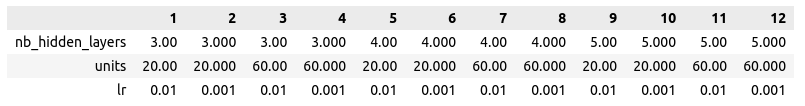
\includegraphics[width=0.7\linewidth]{config_dense.png}
\end{minipage}

On peut représenter de la manière suivante le type de réseau implémenté :

\begin{minipage}{\linewidth}
	\centering
	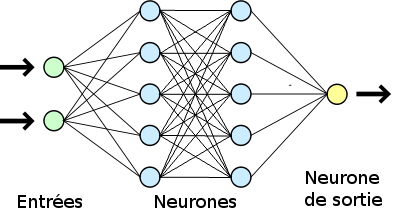
\includegraphics[width=0.4\linewidth]{dense.png}
\end{minipage}

\newpage

\subsection{Modèle 1 : $u=\phi w$}

Dans un premier temps, j'ai implémenté un réseau capable d'apprendre directement la solution $u$. 

\subsubsection{Implémentation du modèle}

Voici les étapes principales effectuées :
\begin{enumerate}[label=\textbullet]
	\item Input X : (nb\_pts,2), Output Y : (nb\_pts,1)  
	\item On crée un modèle keras séquentiel composé de \textit{nb\_hidden\_layers} couche dense de \textit{units} neurones. A noter qu'on rajoute une couche Dense à la fin de 1 neurones.
	\item On compile le modèle en lui donnant un optimiseur (on prend Adam auquel on fournit le taux d'appresntissage \textit{lr}) ainsi que la loss (dans notre cas "mae" fournit par tensorflow).
	\item On fit le modèle à partir de X\_train, Y\_train, une \textit{batch\_size} et un nombre d'époques totales.
\end{enumerate}

\begin{Rem}
	On prendra comme X\_train les coordonnées (x,y) en $\mathbb{P}^2$ avec nb\_vert=32 (pour se ramener au même cas que le FNO) et Y\_train l'évalution de la solution analytique en chacun de ces degrés de liberté.
	
	On sauvegardera également le modèle à différents nombres d'époques sous la forme de checkpoints et à la fin de l'apprentissage, on sauvegardera l'historique (les loss).
\end{Rem}

\subsubsection{Résultats}

On considère ici la solution analytique suivante
$$u_{ex}(x,y)=S\times\sin(2\pi fx+p)\times\sin(2\pi fy+p)$$
avec $S=0.5$, $f=1$ et $p=0$.

\begin{Rem}
	A noter qu'on se place ici dans le cas d'une \textbf{solution non homogène}.
\end{Rem}

On a testé différents modèles. Voici les loss finales obtenus pour chacun des 12 configurations possibles :

\begin{minipage}{\linewidth}
	\centering
	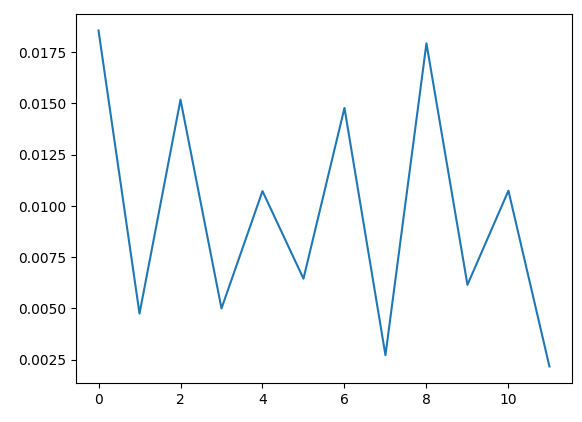
\includegraphics[width=0.4\linewidth]{best_final_loss.png}
\end{minipage}

Il semblerait que les 12 modèles soient plus ou moins capable d'apprendre correctement la solution. On considérera dans la suite le dernier modèle (car c'est celui qui a la meilleure loss finale). On cherche maintenant à corriger la prédiction du modèle 12 en l'injectant dans un solveur PhiFEM. On considère alors la solution en $\mathbb{P}^{10}$ que l'on va corriger par multiplication.

\begin{minipage}{\linewidth}
	\centering
	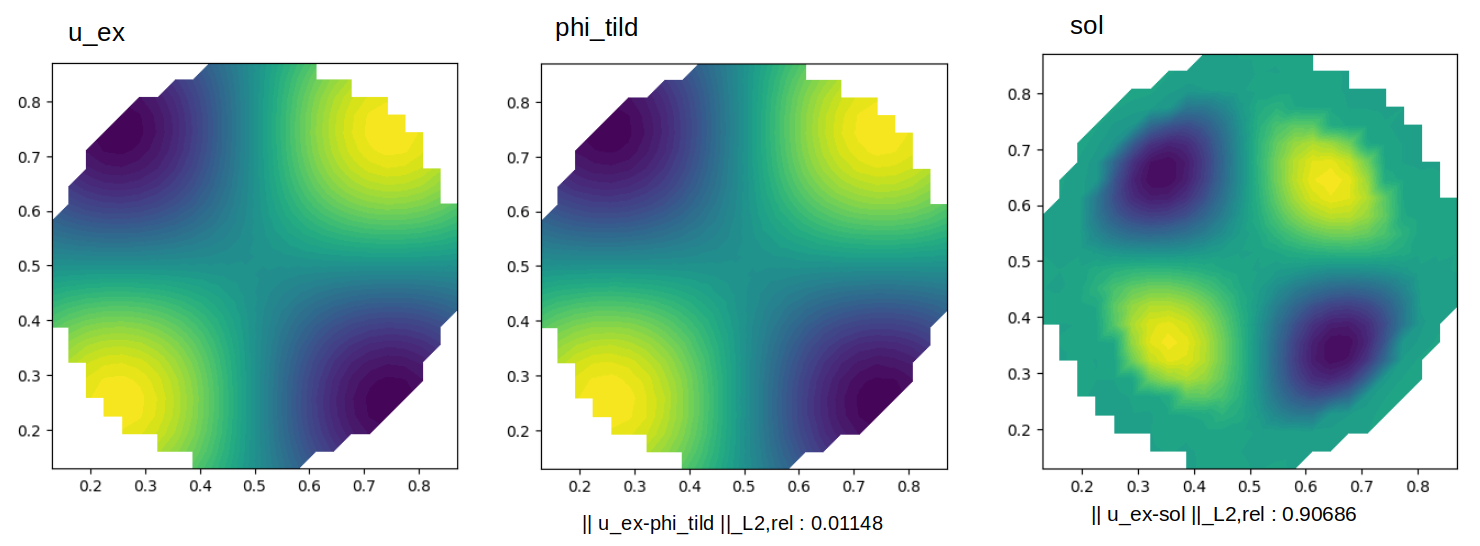
\includegraphics[width=0.7\linewidth]{corr_mod1.png}
\end{minipage}

Il semblerait alors que le solveur ne nous donne pas du tout la bonne solution. Une première hypothèse est que les conditions au bord ne soit pas correctement vérifiées sur phi\_tild et donc C n'est pas imposé faiblement à 1.  

\newpage

\subsection{Modèle 2 : $w$}

Pour être sûre de bien imposer les conditions aux bord, on peut entraîner le modèle à apprendre $w$ plutôt que $u$ et ainsi e multiplier par $\phi$ ensuite (qui est nulle au bord). 

\subsubsection{Implémentation du modèle}

Voici les étapes principales effectuées :
\begin{enumerate}[label=\textbullet]
	\item Input X : (nb\_pts,2), Output Y : (nb\_pts,1)  
	\item On crée un modèle keras séquentiel composé de \textit{nb\_hidden\_layers} couche dense de \textit{units} neurones. A noter qu'on rajoute une couche Dense à la fin de 1 neurones.
	\item On définit une fonction de loss :
\begin{lstlisting}
def loss_mae(y_true,y_pred,xy):
	return tf.reduce_mean(tf.abs(y_true-y_pred*call_phi(None,xy)))
\end{lstlisting}
	ainsi qu'un optimiseur (on prend Adam auquel on fournit le taux d'appresntissage \textit{lr}).
	\item On fit le modèle en utilisant une boucle d'entraînement personnalisée :
	\begin{itemize}
		\item On commence par une première boucle sur les époques.
		\item Pour chaque époque, on shuffle notre X\_train et le Y\_train associé.
		\item On effectue alors une seconde boucle sur les batch dans laquelle on va réaliser une descente de gradient à partir de la loss précédente.
	\end{itemize}
\end{enumerate}

\begin{Rem}
	Comme précédemment, on prendra comme X\_train les coordonnées (x,y) en $\mathbb{P}^2$ avec nb\_vert=32 (pour se ramener au même cas que le FNO) et Y\_train l'évalution de la solution analytique en chacun de ces degrés de liberté.
	
	On sauvegardera également le modèle à différents nombres d'époques sous la forme de checkpoints et à la fin de l'apprentissage, on sauvegardera l'historique (les loss).
\end{Rem}

\subsubsection{Résultats}

On considère ici la solution analytique suivante
$$u_{ex}(x,y)=S\times\sin(2\pi fx+p)\times\sin(2\pi fy+p)\times\cos(4\pi((x-0.5)^2+(y-0.5)^2))$$
avec $S=0.5$, $f=1$ et $p=0$.

\begin{Rem}
	A noter qu'on se place ici dans le cas d'une \textbf{solution homogène}.
\end{Rem}

On a testé les 12 configurations possibles, voici les loss obtenues :

\begin{minipage}{\linewidth}
	\centering
	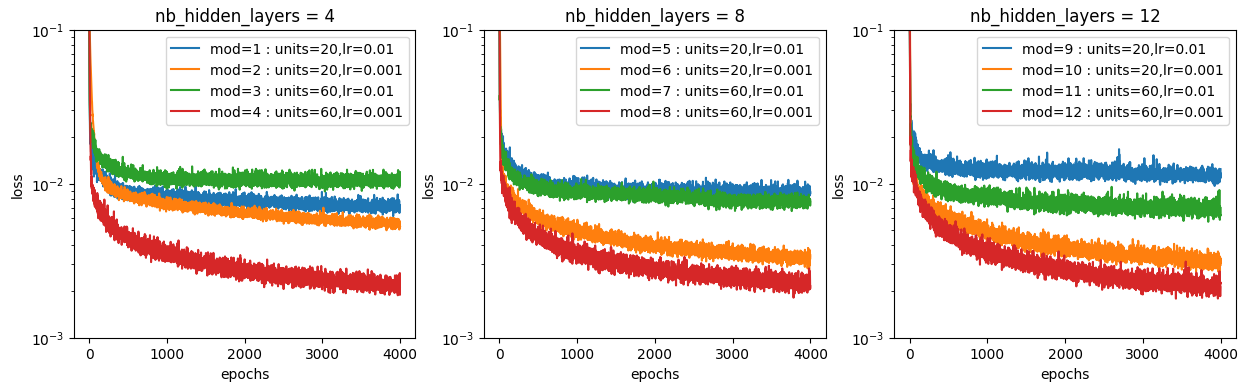
\includegraphics[width=0.9\linewidth]{comp_mod2.png}
\end{minipage}

\begin{Rem}
	Il faudrait rajouter une comparaison des modèles sur un échantillon test !!
\end{Rem}

\newpage


Il semblerait que les 12 modèles soient plus ou moins capable d'apprendre correctement la solution. On considérera dans la suite le modèle 8 (dernier modèle lancé au moment des tests sur la correction). On cherche maintenant à corriger la prédiction du modèle 8 en l'injectant dans un solveur PhiFEM. On considère alors la solution en $\mathbb{P}^{10}$ que l'on va corriger par multiplication.

\begin{minipage}{\linewidth}
	\centering
	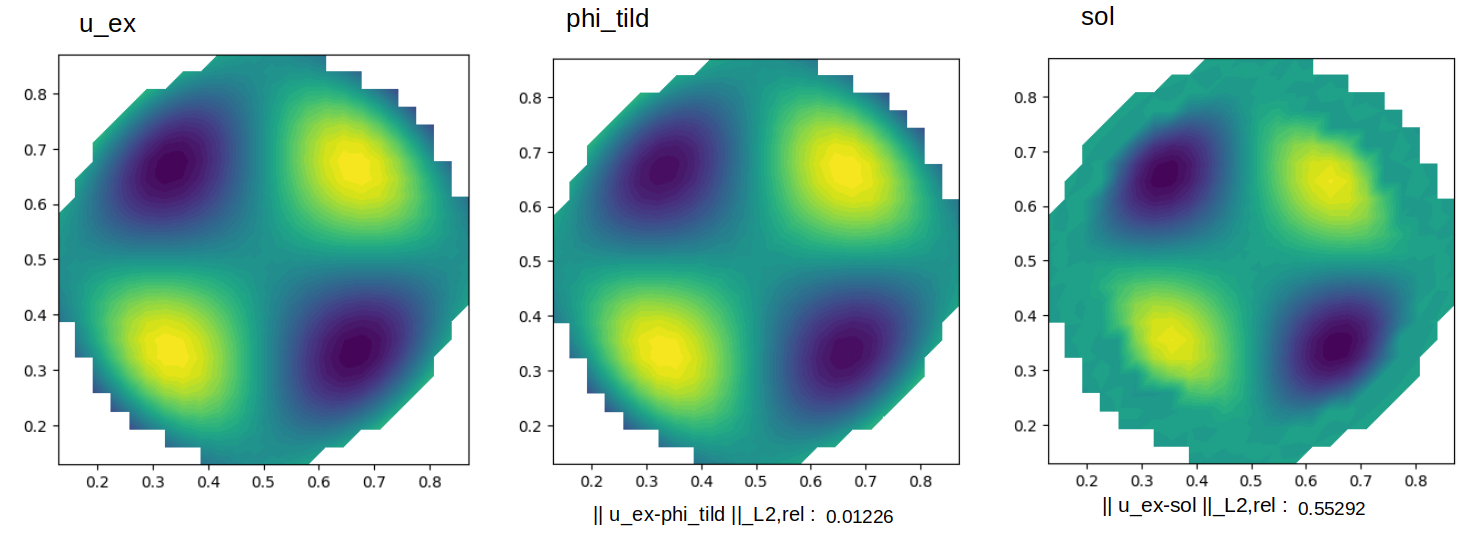
\includegraphics[width=0.7\linewidth]{corr_mod2.png}
\end{minipage}

De la même manière en corrigeant par addition :

\begin{minipage}{\linewidth}
	\centering
	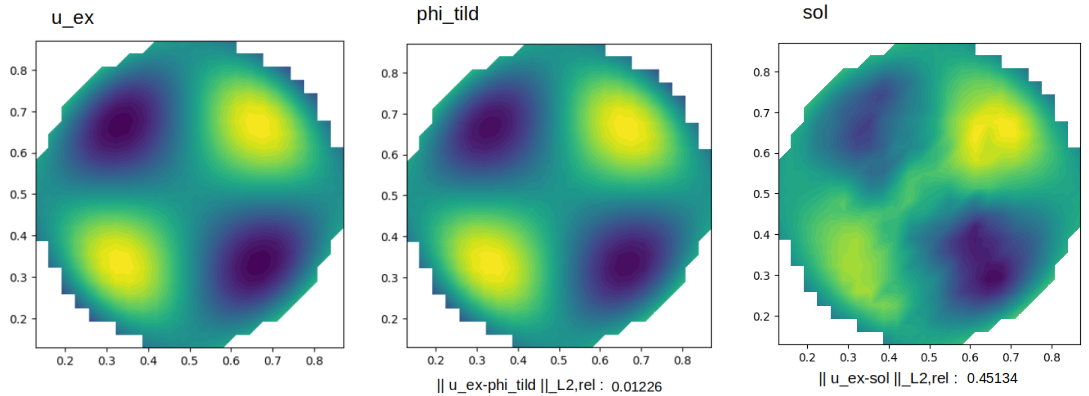
\includegraphics[width=0.7\linewidth]{corr_mod2_add.png}
\end{minipage}

Il semblerait alors que le solveur ne nous donne pas du tout la bonne solution. On dirait que le problème est toujours due au bord mais là c'est bizarre.

\begin{Rem}
	En gardant le même code et en prenant une solution perturbée, on obtient les erreurs attendues. Il semblerait donc que le problème ne vienne pas de là.
\end{Rem}

\subsubsection{Dérivées premières et secondes}

Emmanuel pense que le réseau peut avoir du mal à apprendre les dérivées premières et seconde de la solution et que c'est pour ça que la correction ne fonctionne pas. C'est pourquoi, on va afficher ces informations. Pour cela, on utilmisera la classe implémentée par Vincent Vigon pour le FNO qui permet de calculer les dérivées souhaitées par différences finies.

\begin{minipage}{0.48\linewidth}
	\centering
	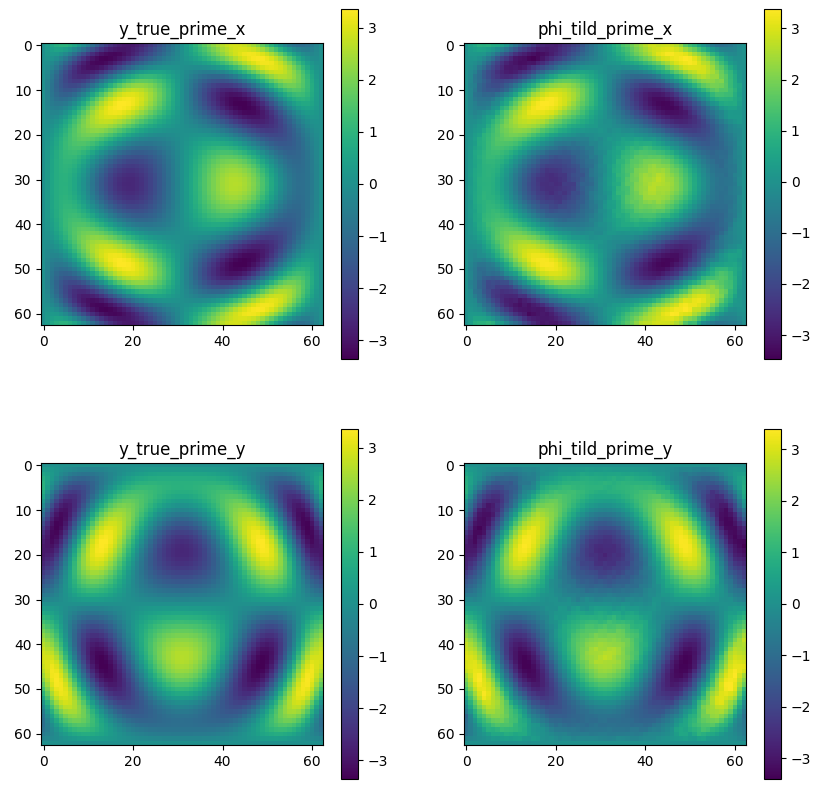
\includegraphics[width=0.9\linewidth]{derivees_premieres.png}
\end{minipage}
\begin{minipage}{0.48\linewidth}
	\centering
	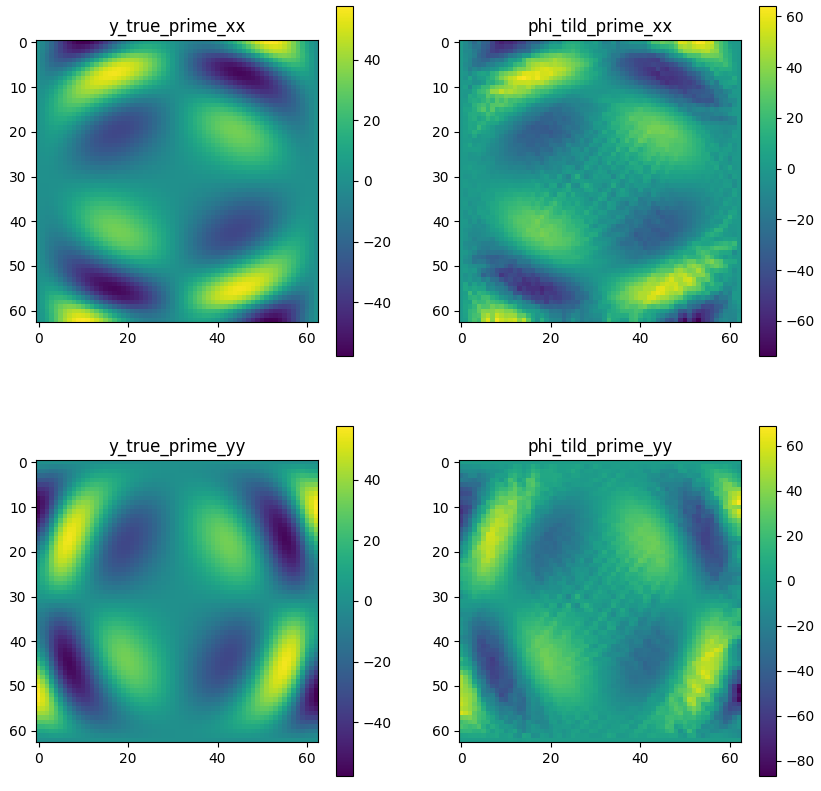
\includegraphics[width=0.9\linewidth]{derivees_secondes.png}
\end{minipage}

\newpage

On calcule également les erreurs en normes $L^2$, $H^1$ et $H^2$ (en directe et pas relative). On considérera ces erreurs sur le carré et sur le cercle. Voici les résultats obtenus :

\begin{minipage}{\linewidth}
	\centering
	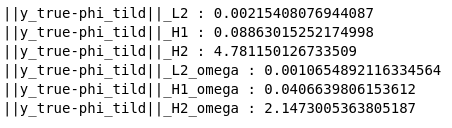
\includegraphics[width=0.5\linewidth]{erreurs.png}
\end{minipage}

\begin{Rem}
	Il semblerait que le réseau ait vraiment du mal à approcher correctement les dérivées secondes.
\end{Rem}


\conclusion{...}